\section*{Motivation and Applications}
\vspace*{-0.1in}
\prob{3}
Since most streaming video became encrypted, which of the following can a network operator {\em no longer read directly} from the traffic, and so must infer? Select all that apply.

\begin{center}
\begin{tabularx}{0.9\textwidth}{X X}
\correctanswercircle{Video resolution} &
\answercircle{Packet sizes and timing}
\\
\correctanswercircle{Rebuffering (stall) events} &
\answercircle{IP addresses of the video servers}
\\
\correctanswercircle{Startup delay before playback} &
\answercircle{Number of parallel connections}
\end{tabularx}
\end{center}
\eprob

\prob{2}
In Hands-On 1 you looked at a packet capture before doing anything else with it. Which observations should make you suspect a problem with the data? Select all that apply.

\begin{center}
\begin{tabularx}{0.9\textwidth}{X X}
\correctanswercircle{A packet with a negative length} &
\answercircle{Large packets flow mostly server to client}
\\
\correctanswercircle{A packet far above the maximum packet size} &
\answercircle{A handshake before the large packets}
\\
\correctanswercircle{Timestamps that go backwards} &
\answercircle{Round-trip times that vary over the trace}
\end{tabularx}
\end{center}
\eprob

\prob{3}
Attackers are preparing a phishing campaign that imitates the University's login page. You run the campus network and can obtain domain registration data and the logs of the campus DNS resolver. Name {\bf one} data source and {\bf two} features you would use to detect the campaign, ideally before the first email arrives.

\answerbox{1.3}{Domain registration data: a burst of newly registered domains at once; names that are close to (a small edit distance from) uchicago.edu; very recent registration date; hosting in a place that makes no sense for the audience. DNS resolver logs: campus clients looking up domains that are only days old or that resemble University names. Email logs also acceptable: sending volume, recipients per message, unusual hours, the sending server's IP geolocation (distance from the recipients), the sender's AS or BGP route. One source, any two sensible features.}
\eprob

\prob{3}
In Hands-On 2, the Log4j scan and the normal web trace were captured at different times of day, so a model with time of day as a feature separates them perfectly. Is time of day a good feature for detecting scans?
\framebox{
\yesnono
}

Why or why not?

\answerbox{1.2}{No. It is an artifact of how this dataset was collected, not of the behavior: scans and normal browsing happen at any hour, so the model would fail on new traffic. One correct reason earns full credit. (Not required, since the question did not ask: features that reflect real differences in behavior, such as short sessions, little large server-to-client content, many unique destinations, different inter-arrival times.)}
\eprob

\section*{Data Acquisition}
\vspace*{-0.1in}
\prob{3}
Which of the following are {\em passive} measurements? Select all that apply.

\begin{center}
\begin{tabularx}{0.95\textwidth}{X X}
\correctanswercircle{An ISP collects flow records from its routers} &
\answercircle{An app downloads a test file every hour}
\\
\correctanswercircle{Campus logs every query its DNS resolver answers} &
\answercircle{A laptop pings a server once a minute}
\\
\correctanswercircle{Inferring resolution from a capture of your Netflix session} &
\answercircle{Measuring latency while a test upload runs}
\end{tabularx}
\end{center}
\eprob

\prob{3}
A student reports that Zoom was choppy half an hour ago. You run a speed test from their laptop now and it reports high throughput and low latency. Does this show the network was not the cause?
\framebox{
\yesnono
}

Why or why not?

\answerbox{1.2}{No. Any one correct reason earns full credit: the active test measures conditions now, and the problem may have been transient; it measures the path to the speed-test server, not to Zoom; it may be limited by Wi-Fi or the device rather than the network; an active test does not reflect what the user experienced. (Not required, since the question did not ask: passive data from the time of the problem, such as flow records or a capture, reflects what the user actually experienced.)}
\eprob

\prob{3}
(a) Name the five header fields that define a flow. In Hands-On 5 it was safe to group packets by only four of them; which one could be left out, and why? (b) Two packets match on all five fields but arrive 45 seconds apart with no packets in between. Would a router using conventional settings put them in the same flow record? Why or why not?

\answerbox{1.3}{(a) Source IP, destination IP, source port, destination port, protocol. Protocol could be omitted because the whole trace was UDP DNS traffic on port 53. (b) No. Routers end a flow after a period of inactivity (typically about 15 to 30 seconds), so the second packet starts a new flow record.}
\eprob

\section*{Features and Representation}
\vspace*{-0.1in}
\prob{4}
In Hands-On 6 you used {\tt netml} to turn a capture into per-flow STATS features. nPrint instead turns each packet into a fixed-width bitmap of its header bits and lets a model learn which bits matter. Give {\bf one advantage} and {\bf one disadvantage} of {\em each} approach.

\answerbox{1.6}{Manual features (netml): advantages are compact input, interpretability, encoding domain knowledge, and the ability to express rates and timing; disadvantages are that it needs domain expertise, many encoding choices hurt reproducibility, and features built for one task may not transfer. Representation learning (nPrint): advantages are no hand-crafted features, one representation reused across tasks, the model finds informative header bits; disadvantages are large storage (about twice), no notion of time or rates, needs more data, and risk of spurious correlations (TTL, addresses) that domain knowledge must catch.}
\eprob

\prob{2}
A flow's protocol is TCP, UDP, or ICMP, and you encode it as 0, 1, 2. Which statements are true? Select all that apply.

\begin{center}
\begin{tabularx}{0.95\textwidth}{X X}
\correctanswercircle{This is usually fine for a random forest} &
\answercircle{Min-max scaling fixes it for a linear model}
\\
\correctanswercircle{A linear model treats ICMP as ``twice'' UDP} &
\answercircle{Tree models require one-hot inputs}
\\
\correctanswercircle{One-hot encoding gives three binary columns} &
\answercircle{The order 0, 1, 2 carries real meaning}
\end{tabularx}
\end{center}
\eprob

\prob{3}
Some rows in your flow dataset have missing values. Give {\bf one} example from network data where filling in the column average is reasonable, and {\bf one} where it is a bad idea. Explain why for the second.

\answerbox{1.3}{Reasonable: a missing measurement in an otherwise steady series where the gap is a recording glitch; a numeric field that clusters tightly, such as packet sizes near the MTU; latency or throughput during a stable period. Bad idea, with why: when the missing or strange value may itself be the anomaly you want to detect (a corrupted sequence number, a malformed packet, an absent field during an attack), averaging erases exactly that signal; a categorical or discrete field (protocol, port, TCP flags, a resolution label), where the average is a value that does not exist; an ordered series such as timestamps or inter-arrival times, where the column mean ignores order (fill from neighbors instead) and hides bursts; computing the average over the whole dataset before the split (leakage). A reason is required only for the bad example.}
\eprob

\section*{Training and Evaluation}
\vspace*{-0.1in}
\prob{3}
You have six months of hourly traffic volumes and want to forecast next month's load to decide whether to add a server. You shuffle all rows randomly, split 80/20, and get low test error. Is that a trustworthy estimate of how well the model will forecast?
\framebox{
\yesnono
}

Why or why not?

\answerbox{1.2}{No. A random split puts later hours in the training set and earlier hours in the test set, so the model predicts the past from the future (temporal leakage); hourly rows are not independent. One correct reason earns full credit. (Not required, since the question did not ask: train on the earlier months and test on the later ones, which also mimics the real forecasting task.)}
\eprob

\prob{5}
A detector labels 1,000 flows; 20 of them are attacks (attack is the positive class). Its confusion matrix:

\begin{center}
\begin{tabular}{r|c|c|}
\multicolumn{1}{c}{} & \multicolumn{1}{c}{Predicted attack} & \multicolumn{1}{c}{Predicted benign} \\ \cline{2-3}
True attack & 15 & 5 \\ \cline{2-3}
True benign & 15 & 965 \\ \cline{2-3}
\end{tabular}
\end{center}

(a) Compute accuracy, precision, and recall. (b) What is the accuracy of a classifier that always says ``benign''? What does the comparison tell you, and which curve would you use to compare detectors on this data?

\answerbox{1.8}{(a) Accuracy = (15+965)/1000 = 98\%. Precision = 15/(15+15) = 50\%. Recall = 15/(15+5) = 75\%. (b) Always-benign: 980/1000 = 98\%, the same accuracy while catching no attacks. Under class imbalance accuracy is misleading; use precision and recall, and the precision-recall curve rather than ROC.}
\eprob

\prob{3}
The figure shows training and validation error as model complexity increases.

\begin{center}
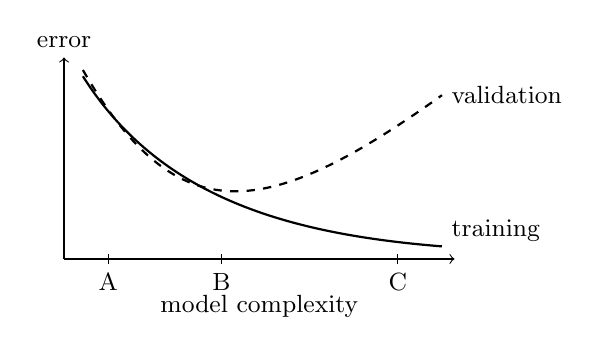
\begin{tikzpicture}[scale=0.8]
\draw[->] (0,0) -- (6.2,0);
\node at (3.1,-0.75) {\small model complexity};
\draw[->] (0,0) -- (0,3.2) node[above] {\small error};
\draw[thick] (0.3,2.9) .. controls (1.5,1.0) and (3.5,0.4) .. (6,0.2);
\node[right] at (6,0.45) {\small training};
\draw[thick,dashed] (0.3,3.0) .. controls (1.8,0.4) and (3.2,0.6) .. (6,2.6);
\node[right] at (6,2.6) {\small validation};
\foreach \x/\l in {0.7/A,2.5/B,5.3/C} {\draw (\x,0.08) -- (\x,-0.08) node[below] {\small \l};}
\end{tikzpicture}
\end{center}

(a) Which point (A, B, C) has high bias? (b) Which is overfitting? (c) Name one way to reduce overfitting other than choosing a simpler model.

\answerbox{1.3}{(a) A (underfitting: high error on training and validation). (b) C (training error keeps falling while validation error rises). (c) More training data, regularization, early stopping, or an ensemble; k-fold cross-validation to tune regularization or depth is also accepted. B is the model to choose, picked with the validation set, never the test set.}
\eprob

\newpage
\section*{Assignment 1: Video Quality Inference}
\vspace*{-0.1in}
\prob{3}
In Hands-On 3 and Assignment 1 you computed a segment-download-rate feature from encrypted Netflix traffic. (a) How can you find segment boundaries without decrypting anything? (b) Why do segments carry information about resolution?

\answerbox{2.0}{(a) The player downloads segments in bursts; boundaries show up as gaps in the download marked by small or zero-byte packets between bursts. Either the bursts and gaps or the small packets alone is a full answer. (b) Adaptive streaming encodes the video at several bitrates; the player requests each segment at a chosen bitrate, so higher resolution means more bytes per segment, which shows up in segment sizes and download rate. Also correct: segments have roughly constant duration, so the bytes per segment reveal the bitrate, and with it the resolution.}
\eprob

\prob{4}
A student's Assignment 1 classifier scores 75\% accuracy with a random train/test split, but about 30\% when every session from one household is held out for testing. (a) What does this suggest the model learned? (b) An ISP wants to deploy the model in new homes. Which accuracy is the better estimate, and name one change that would help.

\answerbox{2.5}{(a) Some features fingerprint the household (its devices, access link, network conditions) rather than video quality; with a random split the same households appear in training and test, so the model can recognize the home instead of the resolution (a spurious correlation, non-representative training data). (b) The held-out-household number. Remove household-specific proxy features, split by household, train on more diverse households (``more data'' counts when it means more households), or balance the classes.}
\eprob

\section*{Feedback}
\vspace*{-0.25in}
\prob{3}
Interest (1=Boring!; 10=Amazing!):
\shortanswerbox{0.5}{7}
Difficulty (1=Too easy; 10=Too hard):
\shortanswerbox{0.5}{6}

One thing you like. One suggestion for improvement:

\answerbox{1.0}{1. The hands-ons. 2. More office hours.}
\eprob
